%\documentclass[journal=jctcce,manuscript=article, layout=twocolumn]{achemso}
\documentclass[journal=jctcce,manuscript=article]{achemso}
\usepackage[table]{xcolor}
\usepackage{amsmath}
\usepackage{amsfonts}
\usepackage{graphicx}
\usepackage{float}
\graphicspath{ {./FIGs/} }

\author{Niccol\`{o} Ricardi}
\email{Niccolo.Ricardi@unige.ch}
\author{Cristina E. Gonz\'{a}lez-Espinoza}
\email{Cristina.GonzalezEspinoza@unige.ch}
\author{Tomasz Adam Weso\l{}owski}
\email{Tomasz.Wesolowski@unige.ch}
\affiliation[University of Geneva]
{Department of Physical Chemistry, University of Geneva, Geneva (Switzerland)}

\title[Negativity of the target density]
  {Negativity of the target density in practical Frozen-Density Embedding Theory based calculations\\
  version April 2, 2022 by TW}

\newcommand{\nr}[1]{\color{red}#1\color{black}}    
\begin{document}

\begin{tocentry}

TOC to be made. Probably isosurfaces of target density.

\end{tocentry}

\begin{abstract}
The accuracy of any observable derived from multi-scale simulations based on Frozen-Density Embedding Theory (FDET) is affected by two inseparable factors: {\it i}) the approximation for the bi-functional ${E}_{xcT}^{nad}[\rho_A,\rho_B]$ representing the non-additivity of density functionals for the exchange-, correlation-, and kinetic  energies and  {\it ii}) the possible violation of the non-negativity condition of the target density for a given density associated with the environment $\rho_B(\mathbf{r})$.

The relative significance of theses two factors is investigated for four representative weakly bound intermolecular clusters and various choices for $\rho_B(\mathbf{r})$.
It is shown that  the violation of the non-negativity condition of the target density is the principal source of error in the FDET energy
if $\rho_B(\mathbf{r})$ corresponds to the isolated environment.
Reduction of both the magnitude of the violation of the non-negativity condition and the error in the FDET energy can be pragmatically achieved by explicit treatment of the electronic polarisation of the environment.

{\color{red} Still to be done in the main manuscript:
1) double check notation; b) don't use capitalisation in the names of the molecules, 3) do not use capitalisation in Kcal/mol
4) TOC if the journal requests it, 5) general spelling and grammar check, 6) specific requests to NR indicated in the manuscript, 7) double check all numbers explicitly discussed in the text
} 
\end{abstract}


\section{Introduction}
The formal framework of 
Frozen-Density Embedding Theory (FDET) provides the basis of multi-scale/multi-level simulation methods that use a multiplicative embedding operator. The self-consistent expressions for the functional for the total energy and the corresponding functional for embedding potential are available for  various possible quantum descriptors of the embedded species \cite{Wesolowski1993,Wesolowski2008,Pernal2009,Wesolowski2015,Wesolowski2020}. 
The environment is described by means of the electron density $\rho_B$ whereas the embedded species by means of the 
embedded $N_A$-electron wavefunction ($\Psi_A$). The total energy of a system is given by the functional ${E}_{v_{AB}}^{FDET}[\Psi_{A},\rho_B]$ which is closely related to the Hohenberg-Kohn energy functional ($E_v^{HK}[\rho]$) known in density-functional theory \cite{Hohenberg1964} formulation of quantum $N$-electron problem (see Eq \ref{eq:nfund} below).

Any multi-level simulation based based on the formal framework of FDET, hinges on two types of approximations/assumptions.
One concerns the used approximation for one of the components of ${E}_{v_{AB}}^{FDET}[\Psi_{A},\rho_B]$ the other concerns the approach to generate $\rho_B$. In FDET, multi-level mean that  $\rho_B$ is generated using other methods than the methods used to optimise $\Psi_A$. The errors due to these two types of approximations combine and their relative significance cannot be determined  in a straightforward matter. The approximation used for ${E}_{v_{AB}}^{FDET}[\Psi_{A},\rho_B]$ leads to errors in the electron density obtained and in errors in energy. The latter can be either positive and negative. The errors due to  $\rho_B$ are always non-negative.
The optimal electron density of the embedded species obtained in FDET ($\rho_A$) is always $v$-representable. 
As a result, if $\rho_B$
is larger than the exact ground-state density of the whole system ($\rho_{AB}$) on some volume element, the sum of $\rho_A$ and
$\rho_B$ cannot be equal to $\rho_{AB}$. As a consequence of the second Hohenberg-Kohn theorem, FDET can only provide the upper bound of the exact ground-state anergy of the whole system. The necessary condition to reach the ground-state energy in FDET calculations is non-negativity of the difference $\rho_{AB}-\rho_B$ on all non-zero volume elements.
We will refer to this difference as the {\it target density}.
The condition of non-negativity of $\rho_{AB}-\rho_B$ cannot be verified in practice because it requires the {\it a priori} knowledge of 
$\rho_{AB}$.

The principal question addressed in the present work is:  {\it Does violation of the non-negativity condition matter in practice?}  
The issue has not been studied systematically in the literature.
Wesolowski and Savin analysed the errors due to approximations used for ${E}_{v_{AB}}^{FDET}[\Psi_{A},\rho_B]$ in a model system for which the exact solutions of FDET are available. Only such densities $\rho_B$  were considered, for which the non-negativity condition was not violated  \cite{Wesolowski2013}. 

The present work reports the result of a computational experiment on a four intermolecular clusters, in which the relative significance 
of the two factors affecting the FDET results is determined. In such an experiment the density and the energy of the whole cluster $\rho_{AB}$ can be evaluated using an adequate method of quantum chemistry and used as a reference for various choices made for $\rho_B$.
In particular, the relation between the violation of the condition of non-negativity of  $\rho_{AB}-\rho_B$  and the electronic polarisation of the environment due to the interactions with the embedded species is investigated.
Fux et al. \cite{Fux2010}, demonstrated that the violation  is minor and only due to numerical effects.
{\color{red}TW to NR: How the violation was measured to justify the statement that it was minor? The effects on what? In which systems? } 

The chosen clusters were considered previously in our study of complexation induced shifts in the excitation energies \cite{Ricardi2018} which showed a remarkably good performance of the used FDET based method despite the fact that the density of the isolated molecule(s) belonging to the environment was used as $\rho_B$  for each electronic excited state. This could be the result of: {\it a})  fortuitous cancellations of errors due to the violation of the non-negativity condition in different electronic states, {\it b}) numerical insignificance of the violation of the non-negativity condition on the total energy, or {\it c}) both. 
For this reason, the present work focusses on one electronic state - the ground-state.
%To this end, we analyzed the 4 systems from Ref.~\citenum{Ricardi2018}, 
The complexes selected for the present study  display different strength of interaction, number of molecules in the environment, number of non-covalent interactions, and the electric charge of the environment:
{\it i})  7-hydroxyquinoline bound to two methanol molecules (7HQ-2MeOH), {\it ii}) uracil bound to five water molecules (uracil-5H$_2$O), {\it iii}) 7-hydroxyquinoline bound to formate (7HQ-formate), and {\it iv}) benzimidazolide bound to two formic acid molecules (PyrBnz-2HCOOH). 
7HQ-2MeOH and  uracil-5H$_2$O are typical hydrogen bonded complexes involving neutral donor and acceptor molecules. 7HQ-formate and PyrBnz-2HCOOH) represent more peculiar cases. In 7HQ-formate, the environment acts as the hydrogen acceptor and is negatively charged. Moreover, the hydrogen bond distance (1.36 \AA) is comparable to that of its ({\color{red}TW to NR: what is "its covalent bond"?} covalent bond (1.09 \AA). 
%We have discussed in Ref.~\citenum{Zech2018} how this poses a challenge due to the large overlap of the subsystem densities. 
In PyrBnz-2HCOOH, the embedded system (PyrBnz) is a hydrogen acceptor and the atom involved carries a significant negative charge.



\section{Methods}
\subsection{FDET and its extension for non-variational methods}
%\subsubsection{FDET energy functional} 
FDET concerns a system of $N_{AB}$ electrons in an external potential  $v_{AB}(\mathbf{r})$.
For interpretation purposes, it is convenient to split the external potential $v_{AB}(\mathbf{r})$ into components $v_{AB}(\mathbf{r})=v_{A}(\mathbf{r})+v_{B}(\mathbf{r})$. 
The  embedded wavefunction and the total energy obtained from FDET do not depend on such splitting. 
Once $v_{AB}(\mathbf{r})$  is split, $v_{A}(\mathbf{r})$ defines a $N_A$-electron Hamiltonian ($\hat{H}_A$) whereas 
$v_{B}(\mathbf{r})$ defines a $N_B$-electron Hamiltonian ($\hat{H}_B$). 
The  FDET energy functional reads: 
\begin{eqnarray} 
\label{eq:E_FDET_v'}
{E}_{v_A,v_B}^{FDET}[\Psi_{A},\rho_B] = \langle\Psi_{A}\vert \hat{H}_A\vert \Psi_{A}\rangle + E^{HK}_{v_B}[\rho_B] + E^{elst,int}_{v_A,v_B}[\rho_A,\rho_B] + E_{xcT}^{nad}[\rho_A,\rho_B], 
\end{eqnarray}
where {\it i}) $\rho_A(\mathbf{r})=\langle\Psi_A\vert\sum_{i=1}^{N_{A}}\delta(\mathbf{r}_i-\mathbf{r})\vert\Psi_A\rangle$,
{\it ii}) $E^{elst,int}_{v_A,v_B}[\rho_A,\rho_B]$ collects  all classical electrostatic contributions to the interaction energy, and 
{\it iii}) $E_{xcT}^{nad}[\rho_A,\rho_B]$ - the definition of this bi-functional depends on the form of the embedded wavefunction\cite{Wesolowski2008}.
%, {\it iv}) $v_A(\mathbf{r})$ and $v_B(\mathbf{r})$ are 
%two external potentials, and {\it v}) $\hat{H}_A$ is   a $N_A$-electron Hamiltonian defined by the potential $v_A(\mathbf{r})$.

%\subsubsection
%{Relation between the FDET energy functional ($E_{v_{A},{v_B}}^{FDET}[\Psi_{A},\rho_B]$) to the Hohenberg-Kohn energy functional ($E_{v_{AB}}^{HK}[\rho]$}

The FDET energy functional is defined to satisfy the following relation:
\begin{equation}\label{eq:nfund}
\min_{\Psi_A\rightarrow N_A} E_{v_{A},{v_B}}^{FDET}[\Psi_{A},\rho_B] = E_{v_{A},{v_B}}^{FDET}[\Psi^{o}_{A},\rho_B]  = E_{v_{AB}}^{HK}[\rho_A^{o}+\rho_B] \ge E_{v_{AB}}^o,
\end{equation}
where $\rho_A^{{o}}(\mathbf{r})=\langle\Psi_A^{{o}}\vert\sum_{i=1}^{N_{A}}\delta(\mathbf{r}_i-\mathbf{r})\vert\Psi_A^{{o}}\rangle$, $\int\rho_B(\mathbf{r})d\mathbf{r}=N_B$, and $E_{v_{AB}}^o$ is the ground-state energy of the $N_A+N_B$-electron system defined by the potential  $v_{A}(\mathbf{r})+v_{B}(\mathbf{r})$.

%\subsubsection{Equation for the stationary embedded wavefunction}
If the density $\rho^{o}_{AB}-\rho_{B}$ is $v$-representable,  $\rho_A^{o}$ defined in Eq. \ref{eq:nfund} can be obtained from the Euler-Lagrange equation:
\begin{eqnarray}
    \left( \hat{H}_A + \hat{v}_{emb}^{{FDET}}[\rho_A^{{o}}, \rho_B; v_B] \right) \Psi_A^{{o}} &=& \lambda^{o}\Psi_A^{{o}} \label{eq:FDET_SE} 
%\\
%&\downarrow& \nonumber\\
%\rho_A^{{o}}(\mathbf{r})&=&\langle\Psi_A^{{o}}\vert\sum_{i=1}^{N_{A}}\delta(\mathbf{r}_i-\mathbf{r})\vert\Psi_A^{{o}}\rangle\nonumber\\
%&\downarrow& \nonumber\\
%    v_{emb}^{{FDET}}[\rho_A^{{o}}, \rho_B; v_B](\mathbf{r}) = v_B(\mathbf{r}) &+&  \int \frac{\rho_B(\mathbf{r}')}{|\mathbf{r}-\mathbf{r}'|} d\mathbf{r}' 
%    + v_{xct}^{nad}[\rho_A^{{o}}, \rho_B](\mathbf{r}). 
%   \nonumber      
\end{eqnarray}
where $v_{emb}^{{FDET}}[\rho_A,\rho_B; v_B]$
is the FDET embedding potential:
\begin{eqnarray}
v_{emb}^{{FDET}}[\rho_A,\rho_B; v_B](\mathbf{r}) &=& v_B(\mathbf{r}) +  \int \frac{\rho_B(\mathbf{r}')}{|\mathbf{r}-\mathbf{r}'|} d\mathbf{r}'+ \frac{\delta E_{xct}^{nad}[\rho_A,\rho_B]}{\delta\rho_A(\mathbf{r})}.
\label{eq:nFDET_embpot}  
\end{eqnarray}
The term $\frac{\delta E_{xct}^{nad}[\rho_A,\rho_B]}{\delta\rho_A(\mathbf{r})}\equiv v_{xct}^{nad}[\rho_A,\rho_B](\mathbf{r})$ depends on the form of the embedded wavefunction\cite{Wesolowski2008}.
For a single determinant, the FDET expression for $E_{xct}^{nad}[\rho_A,\rho_B]$   includes also the correlation functional $E_c[\rho_A]$  assuring that the optimal embedded density satisfies Eq. \ref{eq:nfund}. 
In the present work,  $E_{xct}^{nad}[\rho_A,\rho_B]$ denotes the functional corresponding to the embedded wavefunction of the Full Configuration Interaction form \cite{Wesolowski2008}, i.e., with this component neglected.
The $\rho_A$-dependency of  $v_{xct}^{nad}[\rho_A,\rho_B](\mathbf{r})$ leads to two 
particular features of Eq. \ref {eq:FDET_SE}: {\it i}) solving it involves an iterative procedure leading to self-consistency and {\it ii}) the Lagrange multiplier $\lambda^{o}$  does not represent the energy.  

The self-consistent potential ($v'_A$) obtained from Eq. \ref {eq:FDET_SE}, in which $\Psi_A$ has a single-determinant form ($\Phi'_A$):
\begin{eqnarray}
v'_A(\mathbf{r})=v_A(\mathbf{r})+v_{emb}^{{FDET}}[\rho'_A,\rho_B; v_B](\mathbf{r})\label{eq:def_v'},
\end{eqnarray}
where $\rho'_A(\mathbf{r})=\langle\Phi'_A\vert\sum_{i=1}^{N_{A}}\delta(\mathbf{r}_i-\mathbf{r})\vert\Phi'_A\rangle$,
defines an auxiliary $N_A$-electron system.

%\subsection{FDET energy using a non-variational embedded wavefunction}

According to the recently derived formula relating the quantities available in methods treating the correlation energy of embedded electrons non-variationally to the Hohenberg-Kohn energy functional (Eq. 38 in Ref. \citenum{Wesolowski2020}): 
\begin{eqnarray} \label{eq:E_FDET_gnovc}
 E_{v_{AB}}^{HK}[\rho_A^{o}+\rho_B] &=& E_{v_{A},{v_B}}^{FDET}[\Phi'^{HF}_{A},\rho_B] + E^{c}_{v'_A} 
 % {E}^{HK}_{v_B}[\rho_B] 
 \\ \nonumber
 &-& E_k[\Delta \rho^{c}_{v'_A}, \rho'^{HF}_A, \rho_B] + O(\Delta\rho)^2, %\\ \nonumber%+ E^{c(MPn\;\mathrm{for}\;n>2)))}_{v'_A} 
 \end{eqnarray}
%\mathrm{where}&& \nonumber\\
where,
\begin{eqnarray}
\label{eq:nkernel}
 E_k[\Delta \rho^{c}_{v'_A}, \rho'^{HF}_A, \rho_B] &=&
  \int \rho'^{HF}_A(\mathbf{r})  \int \Delta \rho^{c}_{v'_A}(\mathbf{r'}) f^{nad}_{xcT}[\rho'^{HF}_A, \rho_B](\mathbf{r},\mathbf{r'})d\mathbf{r'}\mathrm{d}\mathbf{r},\\
  \nonumber \\ \label{eq:def_corrdens}
  \Delta \rho^{c}_{v'_A}(\mathbf{r})&=&\rho^{o}_{v'_A}(\mathbf{r})-\rho'^{HF}_{v'_A}(\mathbf{r})\\
  \nonumber \\
 \label{eq:nf_nad}
 f^{nad}_{xcT}[\rho_A, \rho_B](\mathbf{r},\mathbf{r'}) &=& \frac{\delta^2 E^{nad}_{xcT}[\rho_A, \rho_B]}{\delta \rho_A(\mathbf{r}) \delta \rho_A(\mathbf{r'})}.
\end{eqnarray}
$\rho_A^{o}(\mathbf{r})$ in the left-hand side is the optimal correlated density
%\footnote{$\rho_A^{o}(\mathbf{r})$ is the exact, i.e., correlated electron density. {\color{red}This footnote will be removed.} I give it here to bring it to Nicco' and Cristina's attention.} 
defined in Eq. \ref{eq:nfund}. 
The right-hand-side of Eq. \ref{eq:E_FDET_gnovc} is used to approximate $E_{v_{AB}}^{HK}[\rho_A^{o}+\rho_B]$.
The  $E^{c}_{v'_A}$ and  $E_k[\Delta \rho^{c}_{v'_A}, \rho'^{HF}_A, \rho_B]$
 terms can be evaluated in practice by means of conventional non-variational methods 
applied for an auxiliary system of $N_A$ electrons in the potential $v'_A$ given in Eq. \ref{eq:def_v'}:  {\it i})
the optimal single determinant ($\Phi'^{HF}_{A}$), {\it ii}) the corresponding density ($\rho'^{HF}_{A}(\mathbf{r})$), 
{\it iii}) the correlation energy ($E^{c}_{v'_A}$), and {\it iv}) the change of the density due to correlation ($\Delta \rho^{c}_{v'_A}(\mathbf{r})$).  

{\color{red} TW to TW check if every symbol is defined consistently do not use $\rho'^{HF}_{A}$ but specify that primes refer to single determinants not 
$\Phi'_{A}$ not $\Phi'^{HF}_{A}$.}


For $\Delta\rho$  representing the correlation-induced changes of energy in the exact and in the auxiliary system, 
 $O(\Delta\rho)^2$ collects all second- and higher order contributions to the energy. 
As far as the $E^{HK}_{v_B}[\rho_B]$ component of ${ E}_{v_A,v_B}^{FDET}[\Psi_{A},\rho_B]$ is concerned,
its treatment depends on the method used to generate $\rho_B$ and will be given below.


For a given $\rho_B(\mathbf{r})$,
the FDET interaction energy is given by:
\begin{eqnarray}
E_{int}^{FDET(\rho_B)}=E_{v_{AB}}^{HK}[\rho_A^{o}+\rho_B] - E_{v_A}^{HK}[\rho_A^{isol}] - 
E_{v_B}^{HK}[\rho_B^{isol}] \label{eq:eint0}
\end{eqnarray}
Using for  $E_{v_{AB}}^{HK}[\rho_A^{o}+\rho_B]$ for the right-hand side of Eq. \ref{eq:E_FDET_gnovc} with  neglected $O(\Delta\rho)^2$, results in:
\begin{eqnarray}
E_{int}^{FDET(\rho_B)}&=&
\langle\Phi'^{HF}_{A}\vert \hat{H}_{v_A}\vert \Phi'^{HF}_{A}\rangle + E^{c}_{v'_A}
+ E^{elst,int}_{v_A,v_B}[\rho'^{HF}_A,\rho_B] + {E}_{xcT}^{nad}[\rho'^{HF}_A,\rho_B] \label{eq:eint1}\\
&-&     E_k[\Delta \rho^{c}_{v'_A}, \rho'^{HF}_A, \rho_B]  - E_{v_A}^{HK}[\rho_A^{isol}] + {E}^{HK}_{v_B}[\rho_B]  - 
E_{v_B}^{HK}[\rho_B^{isol}] \nonumber
\end{eqnarray}
In the above equation,  the quantities:  $\Phi'^{HF}_{A}$, $\rho'^{HF}_A$, $E^{c}_{v'_A}$, and $\Delta \rho^{c}_{v'_A}$  depend on $\rho_B(\mathbf{r})$. For the clarity of the notation, this dependency is not indicated explicitly. It is implicitly given through  $v'_A$  that depends on  $\rho_B(\mathbf{r})$ (see Eq. \ref{eq:nFDET_embpot}). 

\subsection{FDET interaction energy}
The subsequent sub-sections concerns application of Eq. \ref{eq:eint1} for different choices for $\rho_B(\mathbf{r})$. 
%Numerical implementation of the above formula depends on the choice made for $\rho_B(\mathbf{r})$ due to the evaluation of the ${E}^{HK}_{v_B}[\rho_B]$ term.
\subsubsection{FDET interaction energy for $\rho_B(\mathbf{r})=\rho_B^{isol}(\mathbf{r})$}
In this case, the last two terms in Eq. \ref{eq:eint1} are equal leading to:
\begin{eqnarray}
E_{int}^{FDET(\rho_B^{isol})}&=&
\langle\Phi'^{HF}_{A}\vert \hat{H}_{v_A}\vert \Phi'^{HF}_{A}\rangle + E^{c}_{v'_A}
+ E^{elst,int}_{v_A,v_B}[\rho'^{HF}_A,\rho_B^{isol}]  \label{eq:eint2}\\
&+& {E}_{xcT}^{nad}[\rho'^{HF}_A,\rho_B^{isol}]     - E_k[\Delta \rho^{c}_{v'_A}, \rho'^{HF}_A, \rho_B^{isol}]  - 
\langle\Phi^{HF}_{A}\vert \hat{H}_{v_A}\vert \Phi^{HF}_{A}\rangle - E^{c}_{v_A}
%E_{v_A}^{HK}[\rho_A^{isol}]  
\nonumber
\end{eqnarray}
where the exact relation $E_{v_A}^o=E_{v_A}^{HK}[\rho_A^{isol}]=\langle\Phi^{HF}_{A}\vert \hat{H}_{v_A}\vert \Phi^{HF}_{A}\rangle + E^{c}_{v_A}$ was used for the energy of the isolated subsystem $A$.

 \subsubsection{FDET interaction energy for  $\rho_B^{v"}(\mathbf{r})$ being the ground-state Hartree-Fock density for some 
 potential $v"(\mathbf{r})$} 
In this case, the numerical value of 
${E}^{HK}_{v_B}[\rho_B^{v"}]-{E}^{HK}_{v_B}[\rho_B^{isol}]\ge 0$ contributes to the interaction energy. 
It approximated as:
\begin{eqnarray}
{E}^{HK}_{v_B}[\rho_B^{v"}]=\langle\Phi"^{HF}_{B}\vert \hat{H}_{v_B}\vert \Phi"^{HF}_{B}\rangle+E^{c}[\rho_B^{v"}] \approx \langle\Phi"^{HF}_{B}\vert \hat{H}_{v_B}\vert \Phi"^{HF}_{B}\rangle+E^{c}_{v"},   \label{eq:evb} 
\end{eqnarray}
where $\Phi"^{HF}_{B}$ is the optimal determinant yielding $\rho_B^{v"}$ (not the Hartree-Fock wavefunction for $N_B$ electrons in the potential ${v_B}(\mathbf{r})$!).

Using the above approximation in Eq. \ref{eq:eint1} leads to:
 \begin{eqnarray}
E_{int}^{FDET(\rho_B^{v"})} 
&=&  \langle\Phi'^{HF}_{A}\vert \hat{H}_{v_A}\vert \Phi'^{HF}_{A}\rangle + E^{c}_{v'_A} + \langle\Phi"^{HF}_{B}\vert \hat{H}_{v_B}\vert \Phi"^{HF}_{B}\rangle  + E^{c}_{v"} \label{eq:eint3}\\ \nonumber
&+& E^{elst,int}_{v_A,v_B}[\rho'^{HF}_A,\rho_B^{v"}] + {E}_{xcT}^{nad}[\rho'^{HF}_A,\rho_B^{v"}]-     E_k[\Delta \rho^{c}_{v'_A}, \rho'^{HF}_A, \rho_B^{v"}]  \nonumber\\
&-& 
\langle\Phi^{HF}_{A}\vert \hat{H}_{v_A}\vert \Phi^{HF}_{A}\rangle - E^{c}_{v_A}
- \langle\Phi^{HF}_{B}\vert \hat{H}_{v_B}\vert \Phi^{HF}_{B}\rangle - E^{c}_{v_B}\nonumber
\end{eqnarray}
where $\Phi^{HF}_{X}$ is the Hartree-Fock wavefunctionand  $E^{c}_{v_X}$ denotes the correlation energy in the system defined by the potential $v_X$ ($X=A$ or $B$).
 \subsubsection{FDET interaction energy for  optimised $\rho_B(\mathbf{r})$}
Optimisation of both $\rho_A(\mathbf{r})$ and $\rho_B(\mathbf{r})$  proceeds by performing an iterative cycle (\textit{freeze-and-thaw},$FAT$) in which the
subsystem $A$ and $B$ exchange their roles  in all FDET equations \cite{Wesolowski1996a}. 
In case of freezing $\rho_A(\mathbf{r})$,  $\rho_B$ is represented be means of an embedded $N_B$ electron single determinant ($\Phi'_B$) that is optimal  for a given $\rho_A$. Let us denote the quantities obtained at the end of such an optimisation with: $v'^{FAT}_A$, $\Phi'^{FAT}_A$, $\rho'^{FAT}_A$, 
 $E^{c}_{v'^{FAT}_A}$, and $\Delta \rho^{c}_{v'^{FAT}_A}$  for the subsystem $A$ and
 $v'^{FAT}_B$ $\Phi'^{FAT}_B$, $\rho'^{FAT}_B$, 
 $E^{c}_{v'^{FAT}_B}$, and $\Delta \rho^{c}_{v'^{FAT}_A}$  for the subsystem $B$. Using this notation, Eq. \ref{eq:eint3} reads: 
 \begin{eqnarray}
E_{int}^{FDET(\rho'^{FAT}_B)} 
&=&  \langle\Phi'^{FAT}_{A}\vert \hat{H}_{v_A}\vert \Phi'^{FAT}_{A}\rangle + E^{c}_{v'^{FAT}_A} + \langle\Phi'^{FAT}_{B}\vert \hat{H}_{v_B}\vert \Phi'^{FAT}_{B}\rangle  + E^{c}_{v'^{FAT}_B} \label{eq:eint4A}\\ \nonumber
&+& E^{elst,int}_{v_A,v_B}[\rho'^{FAT}_A,\rho_B'^{FAT}] + {E}_{xcT}^{nad}[\rho'^{FAT}_A,\rho'^{FAT}_B]-     E_k[\Delta \rho^{c}_{v'^{FAT}_A}, \rho'^{FAT}_A, \rho^{FAT}_B]  \nonumber\\
&-& 
\langle\Phi^{HF}_{A}\vert \hat{H}_{v_A}\vert \Phi^{HF}_{A}\rangle - E^{c}_{v_A}
- \langle\Phi^{HF}_{B}\vert \hat{H}_{v_B}\vert \Phi^{HF}_{B}\rangle - E^{c}_{v_B}\nonumber
\end{eqnarray}




If the subsystems A and B exchange their roles in FDET equations (subsequent \textit{freeze-and-thaw} iteration), the corresponding 
expression reads:
 \begin{eqnarray}
E_{int}^{FDET(\rho'^{FAT}_A)} 
&=&  \langle\Phi'^{FAT}_{B}\vert \hat{H}_{v_B}\vert \Phi'^{FAT}_{B}\rangle + E^{c}_{v'^{FAT}_B} + \langle\Phi'^{FAT}_{A}\vert \hat{H}_{v_A}\vert \Phi'^{FAT}_{A}\rangle  + E^{c}_{v'^{FAT}_A} \label{eq:eint4B}\\ \nonumber
&+& E^{elst,int}_{v_B,v_A}[\rho'^{FAT}_B,\rho_A'^{FAT}] + {E}_{xcT}^{nad}[\rho'^{FAT}_B,\rho'^{FAT}_A]-     E_k[\Delta \rho^{c}_{v'^{FAT}_B}, \rho'^{FAT}_B, \rho^{FAT}_A]  \nonumber\\
&-& 
\langle\Phi^{HF}_{B}\vert \hat{H}_{v_B}\vert \Phi^{HF}_{B}\rangle - E^{c}_{v_B}
- \langle\Phi^{HF}_{A}\vert \hat{H}_{v_A}\vert \Phi^{HF}_{A}\rangle - E^{c}_{v_A}\nonumber
\end{eqnarray}
Following Eq. \ref{eq:E_FDET_gnovc}, both above expressions yield $E_{v_{AB}}^{HK}[\rho'^{FAT}_A+\rho'^{FAT}_B]$ up to the second order terms ($O(\Delta\rho)^2$). 
Adding Eqs. \ref{eq:eint4A} and \ref{eq:eint4B}  and dividing the sum by two yields an expression for the interaction energy that is symmetric upon exchange $A$ and $B$.
\begin{eqnarray}
E_{int}^{FDET(FAT)} 
&=&  \langle\Phi'^{FAT}_{B}\vert \hat{H}_{v_B}\vert \Phi'^{FAT}_{B}\rangle + E^{c}_{v'^{FAT}_B} + \langle\Phi'^{FAT}_{A}\vert \hat{H}_{v_A}\vert \Phi'^{FAT}_{A}\rangle  + E^{c}_{v'^{FAT}_A} \label{eq:eint4}\\ \nonumber
&+& E^{elst,int}_{v_B,v_A}[\rho'^{FAT}_B,\rho_A'^{FAT}] + {E}_{xcT}^{nad}[\rho'^{FAT}_B,\rho'^{FAT}_A] \nonumber \\
&-&    \frac{1}{2}\left(E_k[\Delta \rho^{c}_{v'^{FAT}_A}, \rho'^{FAT}_B, \rho^{FAT}_A]  + E_k[\Delta \rho^{c}_{v'^{FAT}_B}, \rho'^{FAT}_A, \rho^{FAT}_B] \right) \nonumber\\
&-& 
\langle\Phi^{HF}_{B}\vert \hat{H}_{v_B}\vert \Phi^{HF}_{B}\rangle - E^{c}_{v_B}
- \langle\Phi^{HF}_{A}\vert \hat{H}_{v_A}\vert \Phi^{HF}_{A}\rangle - E^{c}_{v_A}\nonumber
\end{eqnarray}
%\end{document}
For exact ${E}_{xcT}^{nad}[\rho_A,\rho_B]$ and exact $E^c_{v}$, all three equations
Eqs. \ref{eq:eint4A}, \ref{eq:eint4B}, and \ref{eq:eint4} yield the same energy.
In practical calculations, 
Eqs. \ref{eq:eint4A} and \ref{eq:eint4B} might yield different numerical results due to the following factors:
{\it i})  the approximation: ${E}_{xcT}^{nad}[\rho_A,\rho_B]\approx \tilde{E}_{xcT}^{nad}[\rho_A,\rho_B]$, 
{\it ii}) approximate treatment of the correlation energy $E^c_{v}$, and {\it iii}) the incompleteness of the used basis sets.
The "symmetrised" expression for the interaction energy (Eq. \ref{eq:eint4}) defines uniquely the interaction energy for practical calculations.
{\color{red}TW to TW:  add Delta O}
\subsection{Measures of errors in density}
As a measure of violation of the non-negativity condition by a given density $\rho_{B}(\mathbf{r})$, the
 parameter $M[\rho_{B}(\mathbf{r})-\rho^{o}_{AB}(\mathbf{r})]$ defined as:
\begin{eqnarray}\label{eq:M}
f(\mathbf{r})&=&\rho_{B}(\mathbf{r})-\rho^{o}_{AB}(\mathbf{r}) \nonumber\\
 M[f] & = & \int f(\mathbf{r})\cdot \Theta(f) \ \mathrm{d}\mathbf{r}, \label{eq:def_M}
 %\\ \nonumber
 % & = & -\int \limits_{\{\rho^t < 0\}} \rho^{t},
\end{eqnarray}
where $\Theta$ is the Heaviside step function, is used.

$M$ is bound $0 \le M\le N_{B}$. At the lower bound ($M=0$), the inequality in Eq. \ref{eq:nfund} is reached (subject of the condition of $N_A$-representability of $\rho^{o}_{AB}-\rho_{B}$. If, additionally,  $\rho^{o}_{AB}-\rho_{B}$ is $v$-representable, the exact solution of Eq. \ref{eq:FDET_SE} yield this density.  At the upper bound ($M=N_{B}$), the densities $\rho_{B}$ and $\rho^{o}_{AB}-\rho_{B}$ do not overlap.

The parameter $P[\rho_A^{Eq.\ref{eq:FDET_SE}}+\rho_B-\rho_{AB}^{o}]$ is used as a measure of the  total density obtained from Eq. \ref{eq:FDET_SE}
for a given $\rho_{B}$. It is defined as: 
\begin{eqnarray}
g(\mathbf{r})&=&\rho^{Eq.\ref{eq:FDET_SE}}_A(\mathbf{r})+ \rho_B(\mathbf{r}) - \rho_{AB}^{o}(\mathbf{r}) \nonumber\\
 P[g] &=& \frac{1}{2} 
 %\cdot 
 \int \vert g(\mathbf{r})  \vert d\mathbf{r}, \label{eq:def_P}
\end{eqnarray}
The factor  $\frac{1}{2}$ in the definition of $P[f]$ results in
the the following relation between $M$ and $P$ (see the Supporting Information):
\begin{equation} \label{eq:P_bound}
 M[\rho_{B} - \rho^{o}_{AB}] \leq P[\rho^{Eq.\ref{eq:FDET_SE}}_A+\rho_B - \rho_{AB}^{o}]  \leq %  \int \rho_{AB}^{o} 
  N_{AB}.
\end{equation} 
$M$ and $P$  are used here to discuss different choices of $\rho_{B}(\mathbf{r})$ in {\it the same} system. 

The numerical values of $M$ and $P$ discussed in the present work use the Hartree-Fock densities evaluated for the whole system  as $\rho^{o}_{AB}$. 
%\newpage
\subsection{Computational Details}
%\subsection{FDET with MP2 treatment of correlation for embedded $N_A$ electrons}
The interaction energy was evaluated according to Eqs. \ref{eq:eint2}, \ref{eq:eint3}, and \ref{eq:eint4} applicable for the corresponding choices for $\rho_B(\mathbf{r})$ using the following approximations:
\begin{eqnarray}
%{E}_{xcT}^{nad}[\rho_A,\rho_B]&\approx& \tilde {E}_{xcT}^{nad}[\rho_A,\rho_B] \\
%v_{xct}^{nad}[\rho_A,\rho_B](\mathbf{r})&\approx&\frac{\delta \tilde{E}_{xct}^{nad}[\rho_A,\rho_B]}{\delta\rho_A(\mathbf{r})}\\
E^{c}_{v}&\approx&E_c^{MP2} \label{eq:appr_ec}\\
\Delta \rho^{c}_{v}(\mathbf{r})&\approx&\rho_v^{MP1}(\mathbf{r})-\rho_v^{HF}(\mathbf{r}) \label{eq:appr_rc}
\end{eqnarray}
For the sake of compactness of the used notation, the methods based on the energy expressions given in this section and the used approximations are referred to as FDET-MP2 in this work. 




$E_{xcT}^{nad}[\rho_A,\rho_B]$ and its functional derivative was approximated using local-density approximation (LDA) for all its components: Thomas-Fermi  \cite{Thomas1927, Fermi1928} for the kinetic energy, Dirac-Slater\cite{Slater1929} for the exchange energy, and the Vosko-Wilk-Nusair \cite{Vosko1980} for correlation energy:
\begin{eqnarray}
{E}_{xcT}^{nad}[\rho_A,\rho_B]&\approx& \tilde {E}_{xcT}^{nad(LDA)}[\rho_A,\rho_B] \\
v_{xct}^{nad}[\rho_A,\rho_B](\mathbf{r})&\approx&\frac{\delta \tilde{E}_{xct}^{nad(LDA)}[\rho_A,\rho_B]}{\delta\rho_A(\mathbf{r})}
\end{eqnarray}
The used approximation neglect the correlation component of the embedding potential applicable for single determinants \cite{Wesolowski2008}, representing thus the case for which the relation given in Eq. \ref{eq:E_FDET_gnovc} applies. 
For a given $\rho_B$, the self-consistent quantities needed in the right-hand side of Eq. \ref{eq:E_FDET_gnovc}: 
optimal embedded single determinant ($\Phi'_A$) and the potential defining the auxiliary system ($v'$), 
were obtained by means of an iterative procedure involving repetitive solution of Eq. \ref{eq:FDET_SE}. 
Maximum five to six iterations are needed to converge the total energy within $10^{-9}$ Hartree. 
%{\color{red} TW to NR: How this threshold compares to the threshold for the energy in the SCF iterations?}
The \textit{freeze-and-thaw} optimisation of $\rho_B$ required 7 to 14 iterations to converge to the same threshold, where
one FAT iteration involves obtaining a self consistent solution of Eq. \ref{eq:FDET_SE} ($\Phi'_A$) followed by
solving a "conjoint" equation, in which the indices $A$ and $B$ are switched. Note that the evaluation of the correlation 
energy is needed only after obtaining the final (consistent with the embedding potential) single determinant. 
The above iterative procedures, were performed using the author's version \cite{CCParser_Ricardi} of CCParser\cite{CCParser_Zech} and CCDatabase\cite{CCDatabase} handling
 the automatic submission of Q-Chem5.4\cite{Qchem54} calculations, parsing, and collecting the results.

The aug-cc-pVDZ basis set atomic basis sets were used in all calculations. 
In FDET, two types of expansions were applied: {\it supermolecular expansion}, in which atomic functions localised on all atoms of the system were used, or {\it monomer expansion}, in which the $\Phi_A$ was constructed using only 
atomic functions centred on atoms defining the potential $v_A$ whereas $\Phi_B$ was constructed using only 
atomic functions centred on atoms defining the potential $v_B$.

{\color{red}TW to NR: complete this part PLS 
The geometries of the investigated complexes where obtained from xxxx yyyy and are reported in Ref. \citenum{paperwithgeometries}.}

Throughout this work, the following convention is used for relating Eq. \ref{eq:FDET_SE} and to the names of the complexes/clusters: AAA is associated with $\Psi_A$ and BBB with $\rho_B$ if the system name is AAA-BBB.
In case of optimisation of $\rho_B$, Eq. \ref{eq:emb_SE} is solved 
iteratively for both subsystems. In subsequent  calculations the indices A and B exchange and the order does not matter.
The \textit{freeze-and-thaw} optimisation starts always with the index being $B$ attributed to subsystem BBB. 
 
Parameters $M$ and $P$ were evaluate using the grid integration implemented in PySCF\cite{PYSCF} 
{\color{red} TW to NR:  quoting \cite{Lebedev1999} it is not enough! Grid is defined not only by the angular distribution of points  (Lebedev concerns this) but also by the radial distribution of points and also on the the choice of weights due to the fact that atomic grids do overlap.}
The plots were prepared using the Python modules: pandas\cite{PANDAS} and matplotlib\cite{Hunter2007}.

\subsection{Explicit treatment of the electronic polarisation of $\rho_B$ in FDET}\label{sect:pol_treat}
%\section{Treatment of polarization} \label{sect:pol_treat}
The interpretation of the electronic polarisation of the environment and its effect on the energy is different in FDET and in the theories of intermolecular interactions such as the Symmetry-Adapted Perturbation Theory \cite{Jeziorski1994}. Whereas it enters as a separate component of the energy in the latter case, its identification in FDET is less straightforward.
At the hearth of this difficulty lies the fact that in FDET, the electronic polarisation of each subsystem is not well-defined. As long as the non-negativity condition for $\rho^{o}_{AB}-\rho_B$ is satisfied, any addition of density to $\rho_B$ is not changing the FDET energy. The partition of the total density and consequently the effect of polarisation of $\rho_B$
is, therefore, not unique. 
In FDET based methods, on the other hand,  ${E}_{xcT}^{nad}[\rho_A,\rho_B]\approx \tilde{E}_{xcT}^{nad}[\rho_A,\rho_B]$. 
Even though $\tilde{E}_{xcT}^{nad}[\rho_A,\rho_B]$
is symmetric with respect to exchanging $A$ with $B$, 
the errors in the potentials  $\tilde{v}_{xcT}^{nad}[\rho_A,\rho_B](\mathbf{r})$ and  $\tilde{v}_{xcT}^{nad}[\rho_B,\rho_A](\mathbf{r})$
 are not the same. 
As a result, the unique pair $\rho_A$ and  $\rho_B$ is usually obtained in the \textit{freeze-and-thaw} calculations. 
Optimisation of $\rho_B$  corresponds thus to two effect which cannot be separated, the possibility to reduce the magnitude of the violation of the non-negativity condition, and lowering the total energy given by an approximated expression differing from the exact one by  $\tilde{E}_{xcT}^{nad}[\rho_A,\rho_B]-{E}_{xcT}^{nad}[\rho_A,\rho_B]$. None of them can be uniquely attributed to the electronic polarisation of $\rho_B$. 

The FDET calculations for $\rho_B=\rho_B^{isol}$, on the other hand, take into account the electronic polarisation implicitly if the two densities $\rho_A(\mathbf{r})$ and $\rho_B(\mathbf{r})$ do overlap. 
Even if $\rho_B$ is frozen, the total density near the subsystem $B$ can be modified by the intermolecular interactions due to its $\rho_A$ component.  Since $\rho_A$
is always positive, such implicit treatment of the polarisation cannot expected to be complete. 
This implicit treatment depends on the used basis set which determines the amount of possible overlap between  $\rho_A$ and $\rho_B$.
Moreover, the optimised density 
$\rho_A$ depends critically on the used $\tilde{v}_{xcT}^{nad}[\rho_A,\rho_B](\mathbf{r})$.  

In view of the above observations, it impossible to attribute the differences between the results obtained using $\rho_B=\rho_B^{FAT}$ and  $\rho_B=\rho_B^{isol}$  exclusively to the electronic polarisation of the environment.
To related these differences to the electronic polarisation of the environment an intermediate technique to generate 
 $\rho_B$ was used.
The effect of intermolecular interactions on 
$\rho_B$ was taken into account explicitly
 by means of polarising it by the electric field generated the isolated subsystem $A$. 
The field was approximated using the net-atomic charges corresponding to the isolated subsystem $A$.  
We refer to $\rho_B$ obtained in this way as a pre-polarised density to reflect the fact that the polarising field is generated by isolated subsystem $A$.
The used net atomic charges are fitted to the electric potential generated by $\rho_A^{isol}$  are obtained using the ChelPG method \cite{Breneman1990}.
The pre-polarised density obtained in this way is denoted with  $\rho_B^{pp(ChelPG)}$.
The electric field generated by the  ChelPG  charges has the same long-distance limit behaviour as the FDET embedding potential.
For the reference purposes,  the charges derived from the Mulliken population analysis \cite{Mulliken1955} were also used.
The corresponding densities are denoted with  $\rho_B^{pp(MC)}$.  
For pre-polarised  $\rho_B$,  the interaction energy is given by Eq. \ref{eq:eint3}.

The comparative analysis of the three approaches to the electronic polarisation within FDET, 
are made only for the monomer expansion. The pre-polarisation by net atomic charges misses the quantum effects due to the Fermi statistics of electrons, which leads to unstable numerical results if the basis set is such that the diffusion of electrons towards the environment possible  \cite{Fradelos2011a,Fradelos2011c}.

\section{Results and discussion}
\subsection{FDET results with optimised $\rho_B$}
The FDET interaction energies  obtained using the optimised $\rho_B$ and the complete set of atomic basis sets (supermolecular expansion) collected in Table \ref{table:SE_FAT} compare well with the reference interaction energies.  
The largest deviation from the reference energy occurs for 7HQ-2MeOH (2.88 kcal/mol representing the relative error of about 16\% relative error). 
For the remaining three complexes, the absolute errors are smaller and the relative errors do not exceed 8\%.
Such good performance of the used approximation for $E_{xcT}^{nad}[\rho_A,\rho_B]$
could be expected based on our previous numerical experience \cite{Wesolowski2003a,Kevorkyants2006,Dulak2007a}. The numerical values of $
\delta E_{int}^{FAT}=E^{FDET(FAT)}_{int}-E_{int}^{ref}\label{eq:def_err_en}$
 can be attributed mainly to the used  approximation for $E_{xcT}^{nad}[\rho_A,\rho_B]$. 
 $\rho_B$ was optimised and the same basis set was used in FDET (embedded MP2) and the reference supermolecular calculations (MP2). 8\%). 
Other factors contributing to the deviations from the reference energies are due to incompleteness of the basis sets and to the higher than second-order contributions to the correlation energy. These effects might not completely cancel each other in FDET and in the reference calculations. 

The non-zero values of  the parameters $P$ and $M$, on the other hand, arise from the used approximation to $v_{xcT}^{nad}[\rho_A,\rho_B]$. 
The closer they are to zero the better is $\tilde{v}_{xcT}^{nad}[\rho_A,\rho_B](\mathbf{r})$.
The numerical values of $P$, $M$, and $\delta E_{int}$ given in Table \ref{table:SE_FAT} are considered in the subsequent discussion as the reference residual due to ${v}_{xcT}^{nad}[\rho_A,\rho_B](\mathbf{r})\approx\tilde{v}_{xcT}^{nad}[\rho_A,\rho_B](\mathbf{r})$ and will be compared to the values obtained upon adding additional approximations concerning  $\rho_B$.

\begin{table*}
{
\begin{center}
\begin{tabular}{|c|c|c|c|c|c|}
\hline
 complex & $P^a$ & $M^b$ & $\delta E_{int}\;^c$&$E^{FDET(FAT)}_{int}$ $^d$&$E_{int}^{ref}$ $^e$ \\ \hline
7HQ-2MeOH &0.059& 0.007 & 2.88 &-14.59 & -17.47 \\ \hline
7HQ-formate &0.066& 0.007 &  2.80&-33.68 & -36.48 \\ \hline
uracil-5H$_2$O &0.114&  0.014 & -1.66&-40.28 & -38.62 \\ \hline
PyrBnz-2HCOOH  &0.104& 0.013 & 1.20&-35.33 &  -36.53 \\ \hline
\multicolumn{6}{c}{ } \\
\multicolumn{6}{l}{$^a$ $M=M[\rho^{ref} - \rho^{FDET(FAT)}_{B}]$ with $M[\rho]$ defined in Eq. \ref{eq:M}}\\
\multicolumn{6}{l}{$^b$ $P=P[\rho^{ref} - \rho_{tot}^{FDET(FAT)}]$ with $P[\rho]$ defined in Eq. \ref{eq:def_P}}\\
\multicolumn{6}{l}{$^c$ $\delta E_{int}=E^{FDET(FAT)}_{int}-E_{int}^{ref}$} \\
\multicolumn{6}{l}{$^d$ $E^{FDET(FAT)}_{int}$ is given in Eq. \ref{eq:eint4}}\\
\multicolumn{6}{l}{$^e$ The reference MP2 interaction energies ($E_{int}^{ref}$) are counterpoint corrected.}
\end{tabular}
\end{center}
}%
\caption{Deviations of the FDET-MP2 results from the reference data.  In FDET, \textit{freeze-and-thaw} optimised $\rho_B$ and the reduced set of atomic basis sets (supermolecular expansion) are used. 
Density measures $M$ and $P$ are given in atomic units, energies in kcal/mol.
}
\label{table:SE_FAT}
\end{table*}

Some analyses in the present work are made using a reduced set of atomic basis sets (monomer expansion). This adds an additional factor contributing to the deviations of FDET interaction energies from the reference ones.  
For the sake of meaningful comparisons, Table \ref{table:ME_FAT} collects the FDET results obtained with optimised $\rho_B$ but evaluated using the monomer expansion.

\begin{table*}
{
\begin{center}
\begin{tabular}{|c|c|c|c|c|c|}
\hline
 complex & $P^a$ & $M^b$ & $\delta E_{int}\;^c$&$E^{FDET(FAT)}_{int}$ $^d$ &$E_{int}^{ref}$ $^e$ \\ \hline
7HQ-2MeOH &0.073& 0.013 & 4.00 &-13.47 & -17.47 \\ \hline
7HQ-formate &0.114& 0.036 &  8.21&-28.27 & -36.48 \\ \hline
uracil-5H$_2$O &0.129&  0.024 & 0.94&-37.68 & -38.62 \\ \hline
PyrBnz-2HCOOH  &0.127& 0.016  & 3.74&-32.79 &  -36.53 \\ \hline
\multicolumn{6}{c}{ } \\
\multicolumn{6}{l}{$^a$ $M=M[\rho^{ref} - \rho^{FDET(FAT)}_{B}]$ with $M[\rho]$ defined in Eq. \ref{eq:M}}\\
\multicolumn{6}{l}{$^b$ $P=P[\rho^{ref} - \rho_{tot}^{FDET(FAT)}]$ with $P[\rho]$ defined in Eq. \ref{eq:def_P}}\\
\multicolumn{6}{l}{$^c$ $\delta E_{int}=E^{FDET(FAT)}_{int}-E_{int}^{ref}$} \\
\multicolumn{6}{l}{$^d$ $E^{FDET(FAT)}_{int}$ is given in Eq. \ref{eq:eint4}}\\
\multicolumn{6}{l}{$^e$ The reference MP2 interaction energies ($E_{int}^{ref}$) are counterpoint corrected.}
\end{tabular}
\end{center}
}%
\caption{Deviations of the FDET-MP2 results from the reference data.  In FDET, \textit{freeze-and-thaw} optimised $\rho_B$ and the reduced set of atomic basis sets (monomer  expansion) are used. Density measures $M$ and $P$ are given in atomic units, energies in kcal/mol.
}
\label{table:ME_FAT}
\end{table*}

Limiting the basis set expansion to functions centred on one subsystem increases the interaction energies reflecting thus the variational principle (the total energy decreases). Except for uracil-3H$_2$O, the energies obtained with basis sets centred on all atoms of the complex are closer to the MP2 reference. In the monomer expansion case, the total density obtained as a sum of two subsystem densities, does not include products of  basis functional localised in different subsystems. The largest effect on energy due to neglecting of such terms occurs for 7HQ-formate case (the error increases from 2.88 to 8.21~kcal/mol) - arguably the most covalently bound complex among the four considered in this work. In all cases, the magnitude of the violation of the non-negativity condition ($M$)  is smaller if the {\it supermolecular expansion} is used. 

In practice, for the multi-scale numerical simulations,  optimising 
$\rho_B$ by means of the {\it freeze-and-thaw} iterations is rather not realistic. Such simulations hinge on the possibility to generate $\rho_B$ 
in a simpler/less costly way. 
The subsequent sections concern such applications of FDET. 
To this end, the the deviations from the reference data will be analysed in presence of additional assumptions concerning $\rho_B$ obtained in alternative ways. In particular, the effect of these additional assumptions on the parameter $M$ wiill be discussed.

\subsection{FDET results without optimisation of $\rho_B$: $\rho_B=\rho_B^{isol}$}
%We start with $\rho_B(\mathbf{r})$ obtained from calculations for isolated subsystem B ($\rho_B(\mathbf{r})=\rho_B^{isol}(\mathbf{r})$.)  collected in Tables \ref{table:SE_isol} and \ref{table:ME_isol}

We start with 
%the discussion the FDET results obtained for $\rho_B=\rho_B^{isol}$ and for $\rho_B=\rho_B^{FAT}$ with 
the observation that the {\it  monomer expansion} affects much less the errors in the FDET energies  and densities obtained using the {\it supermolecuar expansion}
than replacing the optimised $\rho_B^{FAT}$ by $\rho_B^{isol}$ (compare the corresponding numerical values in 
Tables \ref{table:SE_FAT},  \ref{table:ME_FAT}, and \ref{table:SE_isol}). 
%The numerical values of these errors are significantly larger if $\rho_B$
%is not optimised. 
The errors in energy ($\delta E_{int}$) and in density ($P$) increase   by a factor of about 2 to 3, whereas the $M$  measuring the extend of the violation of the non-negativity of the target density by the used $\rho_B$ increases  one order of magnitude more (see Tables \ref{table:SE_FAT} and Tables \ref{table:SE_isol}). 

\begin{table*}
{
\begin{center}
\begin{tabular}{|c|c|c|c|c|c|}
\hline
 complex & $P^a$ & $M^b$ & $\delta E_{int}\;^c$&$E^{FDET(\rho_B=\rho_B^{isol})}_{int}$ &$^d$ $E_{int}^{ref}$ $^e$ \\ \hline
7HQ-2MeOH &0.228& 0.121 & 6.27 &-11.20 & -17.47 \\ \hline
7HQ-formate &0.316& 0.206 &  13.14&-23.34 & -36.48 \\ \hline
uracil-5H$_2$O &0.426&  0.234 & 6.15&-32.47 & -38.62 \\ \hline
PyrBnz-2HCOOH  &0.416& 0.184 & 9.36&-27.17 &  -36.53 \\ \hline
\multicolumn{6}{c}{ } \\
\multicolumn{6}{l}{$^a$ $M=M[\rho^{ref} - \rho^{isol}_{B}]$ with $M[\rho]$ defined in Eq. \ref{eq:M}}\\
\multicolumn{6}{l}{$^b$ $P=P[\rho^{ref} - \rho_{tot}^{FDET(\rho_B=\rho_B^{isol})}]$ with $P[\rho]$ defined in Eq. \ref{eq:def_P}}\\
\multicolumn{6}{l}{$^c$ $\delta E_{int}=E^{FDET(\rho_B=\rho_B^{isol})}_{int}-E_{int}^{ref}$} \\
\multicolumn{6}{l}{$^d$ $E^{FDET(\rho_B=\rho_B^{isol})}_{int}$ is given in Eq. \ref{eq:eint2}}\\
\multicolumn{6}{l}{$^e$ The reference MP2 interaction energies ($E_{int}^{ref}$) are counterpoint corrected.}
\end{tabular}
\end{center}
}%
\caption{Deviations of the FDET-MP2 results from the reference data.  In FDET, $\rho_B=\rho_B^{isol}$  and the complete set of atomic basis sets (supermolecular  expansion) are used. 
Density measures $M$ and $P$ are given in atomic units, energies in kcal/mol\\
$^e$ $E^{FDET(rho_B=\rho_B^{isol})}_{int}$ is given in Eq. \ref{eq:eint2}.
}
\label{table:SE_isol}
\end{table*}



\begin{table*}
{
\begin{center}
\begin{tabular}{|c|c|c|c|c|c|}
\hline
 complex & $P^a$ & $M^b$ & $\delta E_{int}\;^c$&$E^{FDET(\rho_B=\rho_B^{isol})}_{int}$ $^d$&$E_{int}^{ref}$ $^e$ \\ \hline
7HQ-2MeOH &0.231& 0.123 & 6.56 &-10.91 & -17.47 \\ \hline
7HQ-formate &0.316& 0.205 &  13.25&-23.23 & -36.48 \\ \hline
uracil-5H$_2$O &0.427&  0.237 & 6.62&-32.00 & -38.62 \\ \hline
PyrBnz-2HCOOH  &0.419& 0.185 & 10.55&-25.98 &  -36.53 \\ \hline
\multicolumn{6}{c}{ } \\
\multicolumn{6}{l}{$^a$ $M=M[\rho^{ref} - \rho^{isol}_{B}]$ with $M[\rho]$ defined in Eq. \ref{eq:M}}\\
\multicolumn{6}{l}{$^b$ $P=P[\rho^{ref} - \rho_{tot}^{FDET(\rho_B=\rho_B^{isol})}]$ with $P[\rho]$ defined in Eq. \ref{eq:def_P}}\\
\multicolumn{6}{l}{$^c$ $\delta E_{int}=E^{FDET(\rho_B=\rho_B^{isol})}_{int}-E_{int}^{ref}$} \\
\multicolumn{6}{l}{$^d$ $E^{FDET(\rho_B=\rho_B^{isol})}_{int}$ is given in Eq. \ref{eq:eint2}}\\
\multicolumn{6}{l}{$^e$ The reference MP2 interaction energies ($E_{int}^{ref}$) are counterpoint corrected.}
\end{tabular}
\end{center}
}%
\caption{Deviations of the FDET-MP2 results from the reference data.  In FDET, $\rho_B=\rho_B^{isol}$  and the reduced set of atomic basis sets (monomer  expansion) are used. 
Density measures $M$ and $P$ are given in atomic units, energies in kcal/mol.
}
\label{table:ME_isol}
\end{table*}

For any choice for $\rho_B$,
the ratio $f[\rho_B]$ defined as:
\begin{eqnarray}
f[\rho_B]=\frac{P[\rho^{ref} - \rho_{A}^{FDET(\rho_{B})}-\rho_{B}]}{P[\rho^{ref} - \rho_{A}^{FDET(FAT)}-\rho_{B}^{FDET(FAT)}]}
\end{eqnarray}
provides a quantitive measure of the relative significance of two factors affecting the total density obtained in FDET:
a) the approximation $v_{xcT}^{nad}[\rho_A,\rho_B]\approx \tilde{v}_{xcT}^{nad}[\rho_A,\rho_B]$  and b) the arbitrary choice of the procedure to generate $\rho_B$ that might lead to such $\rho_B$ that  
$\rho_{AB}-\rho_B$ violates the non-negativity condition.
If the supermolecular expansion is used, the denominator determines the error in the density due to the first factor whereas the numerator arises from the combination of the two of them.
In all considered cases,  $f[\rho_B^{isol}]$ is at least 3.

This observations indicate clearly that  the errors of the FDET results originate mainly due to the violation of the non-negativity condition rather then due to the choice of the used approximation for ${E}_{xcT}^{nad}[\rho_A,\rho_B]$ and ${v}_{xcT}^{nad}[\rho_A,\rho_B](\mathbf{r})$.

We note also that despite a significant increase of the magnitude of the violation of the non-negativity condition in the $\rho_B=\rho_B^{isol}$ case (by at least one order of magnitude), the errors of global properties of the system such as the total density (measured by the parameter $P$) and the interaction energy (measured by $\delta E_{int}$) are affected less. This is probably due to the variational character of densities obtained in FDET.  The error in energy  due to this violation by  the chosen $\rho_B$ is compensated by means of the variationally obtained $\rho_A$.




Comparing the FDET energies obtained using for either $\rho_B=\rho_B^{isol}$ or $\rho_B=\rho_B^{FAT}$ shows clearly that the choice $\rho_B=\rho_B^{isol}$ introduces additional errors in energies. In the FDET terms, the increase of the error is due to a stronger violation of the non-additivity condition for $\rho^{o}_{AB}-\rho_B$ in the former case.


The analyses presented in the present work 
%concern the ground state properties (energy and density) that 
were inspired 
by our previous studies concerning the FDET based simulations of complexation induced shifts of the excitation energies in intermolecular complexes.
{\color{blue}

{\color{red} TW to NR: check the numbers pls the part in blue below is probably the most important message of the whole paper:}


As shown in Ref. \citenum{Ricardi2018}, the $\rho_B=\rho_B^{isol}$ approximation in FDET leads to an astonishingly good overall accuracy of the complexation induced shifts of the vertical excitation energies (errors in the order 0.04~eV). This magnitude of the error in energy is much smaller than the errors reported in Tables \ref{table:SE_isol} and \ref{table:ME_isol}) obtained using the same choice for $\rho_B$. 
According to the present analysis, such a choice for   
$\rho_B$ leads to an error in the ground state energy of at least 6 kcal/mol (equivalent to 0.26 eV).}

The present analysis shows that the violation of the non-additivity condition is a major source of error in the ground-state energy if $\rho_B=\rho_B^{isol}$. Since this error is non-negative regardless of the system (see Eq. \ref{eq:nfund}),
the  much better performance of the $\rho_B=\rho_B^{isol}$ approximation for excitation energies \cite{Ricardi2018},than for the interaction energies has its origin in a systematic compensation of these non-negative contributions to the total energy in two electronic states. 


\subsection{FDET results with pre-polarized  $\rho_B$}

The fact that optimisation of $\rho_B$ not only reduces the errors in the FDET energies but also leads to lowering of the magnitude of violation of the non-negativity condition indicates the link between electronic polarisation of 
$\rho_B$. 
The subsequent part concerns this link and aims at more efficient ways to generate $\rho_B$ than optimising by means of the  {\it freeze-and-thaw} iterations.  
We start with pointing out that using the  {\it monomer expansion} instead of the {\it supermolecular expansion} results in a much smaller effect on the energy than the optimisation of $\rho_B$ in the investigated complexes and with the used $\tilde{E}_{xcT}^{nad}[\rho_A,\rho_B]$. 
Only the  FDET  obtained using the {\it monomer expansion} are, therefore, discussed in this section.
Figure \ref{fig:M_vs_MP} 
%and \ref{fig:M_VS_HF} 
shows the results discussed in the previous sections but also data obtained using other choices  for $\rho_B$.
Pre-polarisation of $\rho_B$ by the field generated by the ChelPG charges corresponding to $\rho_A^{isol}$ leads to lowering of the parameter $M$ and brings it closer to the value of $M$ for the optimised $\rho_B$. 
Lower values of $M$, i.e. less significant violation of the non-negativity condition, correspond also to improved energies. 
The FDET energies obtained using the pre-polarised $\rho_B$ and optimised $\rho_B$ agree within about 1kcal/mol.
Using the  Mulliken charge representation of $\rho_A^{isol}$ does not lead to similar - desired - effects. 
The advantage of using the ChelPG  over the Mulliken charges  in order to polarise $\rho_B$ could be expected.  The former ones are fitted to the electrostatic potential generated by the molecule.
\begin{figure}[H]
\centering
\includegraphics[width=1.0\linewidth]{M_vs_MP_220401.png}
\caption{Integrated negative density $M$ and the FDET-MP2 interaction energy for various choices of $\rho_B$:  a) $\rho_B^{isol}$ (orange triangles), b) $\rho_B^{FAT}$ (light blue hexagons), c) $\rho_B^{pp(Mulliken)}$ (green diamonds), and d) $\rho_B^{pp(ChelPG)}$ (dark blue pentagons). Data obtained using the monomer expansion. Horizontal lies indicate the reference interaction energy.}
\label{fig:M_vs_MP}
\end{figure}

Figure \ref{fig:M_vs_P} shows that the pre-polarisation of $\rho_B$ using the  ChelPG representation of $\rho_A^{isol}$
results also with a significant improvement in the total density.
%\end{document}

\begin{figure}[H]
\centering
\includegraphics[width=1.0\linewidth]{M_vs_P_220401.png}
\caption{Integrated negative density $M$ and the total density error $P$ for various choices of $\rho_B$:  a) $\rho_B^{isol}$ (orange triangles), b) $\rho_B^{FAT}$ (light blue hexagons), c) $\rho_B^{pp(Mulliken)}$ (green diamonds), and d) $\rho_B^{pp(ChelPG)}$ (dark blue pentagons). Data obtained using the monomer expansion.}
\label{fig:M_vs_P}
\end{figure}
% \end{document}


\section{Conclusions}

The present work shows comprehensively that the error in the energy and the density due to the used semi-local approximations for 
${E}_{xcT}^{nad}[\rho_A,\rho_B]$ is significantly  smaller than the error in these quantities due to  the use of the density of the isolated environment as $\rho_B$ in FDET.
This fact lies at the origin of  a  remarkable performance of such FDET based calculations if such density is used  \cite{Ricardi2018}.
Whereas  the approximation  to ${E}_{xcT}^{nad}[\rho_A,\rho_B]$ can result in the error in energy of a given electronic states both negatively or positively, the error in energy due to  such a choice for $\rho_B$ on the energy 
is always non-negative (see Eq. \ref{eq:nfund}). The origin of the good description of vertical excitation energies lies, therefore, in a systematic cancellation of these non-negative contributions for each state.

For the energy of one state, on the other hand, there is no other component that could compensate an error due to violation of this condition. In practical calculations, verification  of the condition of the non-negativity of $\rho^{o}_{AB}-\rho_B$ is not possible. This would require a prior knowledge of the total density.
The present work provided a link between the violation of the condition of the non-negativity of $\rho^{o}_{AB}-\rho_B$
and the effect of electronic polarisation of $\rho_B$ by the embedded species. Due to this link, the magnitude
of the violation of the non-negativity condition of $\rho^{o}_{AB}-\rho_B$ can be significantly reduced  in practice.

%\newpage
%
%$\;$


%\end{document}

\begin{suppinfo}
{\color{red} TW to NR: 
SI should comprise the following information

The data is provided in csv.
\begin{itemize}
  \item Filename: data as comma separated values. The labels are explained below:
  \begin{itemize}
   \item label: explanation
  \end{itemize}
  \item Appendix about the relation between M to P
  \item BSSE
  \item kernel contributions
\end{itemize}
}
\end{suppinfo}

%\end{document}


%%%%%%%%%%%%%%%%%%%%%%%%%%%%%%%%%%%%%%%%%%%%%%%%%%%%%%%%%%%%%%%%%%%%%
%% The appropriate \bibliography command should be placed here.
%% Notice that the class file automatically sets \bibliographystyle
%% and also names the section correctly.
%%%%%%%%%%%%%%%%%%%%%%%%%%%%%%%%%%%%%%%%%%%%%%%%%%%%%%%%%%%%%%%%%%%%%
\bibliography{group_bibliography}

\end{document}



A similar  analysis to that concerning  FDET-MP2 made for of the  FDET-HF component of the FDET-MP2 energy (and the corresponding Hartree-Fock reference) reveals the trends in line with the ones found for  FDET-MP2 (see Supporting Information) and will not be discussed further here.




Figure \ref{fig:N_vs_HF_SE} shows also that the FAT iterations converge rapidly. 
Further optimisation of 
$\rho_B$ beyond the  first one is not needed in practice in the case of the two typical hydrogen-bonded complexes. 
In the case of more strongly bound complexes (7HQ-formate and PyrBnz-2HCOOH), going beyond the first optimisation  of $\rho_B$ affects the total energy only marginally {\color{red}NR: maybe the numbers should be given here - absolute or relative contributions to the interaction energy for instance}.

The behaviour of $M[\rho^{ref} - \rho^{FT,n}_{B}]$ and $P[\rho^{o}_A, \rho_B, \rho^{ref}]$ along the freeze-and-thaw iterations is very similar to that of the energy (see the Supporting Information).


\subsection{FDET energy along the freeze-and-thaw optimisation of $\rho_B$}
% \subsection{Freeze and Thaw cycles}
The numerical procedure used to optimise $\rho_B$  yields a series of intermediate densities 
$\rho_B^{FAT,n}(\mathbf{r})$, providing thus additional set of data for the analysis of the relation between the non-negativity violation and the errors in the energy. $N$ optimisation cycles, provide $\frac{N}{2}$ intermediate densities $\rho_B^{FAT,n}(\mathbf{r})$.  Moreover, the intermediate numerical results make it possible to demonstrate the numerical performance of the $\tilde{E}_{xcT}^{nad}[\rho_A,\rho_B]$. In conventional FDET calculations, obtaining the 
FDET-HF component of the FDET-MP2 energy involves an iterative procedure leading to the optimal single determinant which is consistent with the embedding potential. Linearisation makes it possible to eliminate these iterations.
At each even-numbered iteration, i.e.,  for a given $\rho_B^{FAT,n}(\mathbf{r})$,  the FDET-HF energy  was evaluated in two ways: {\it i}) conventionally way, in which  additional iterations were used to make the embedding potential 
and the embedded single determinant consistent, and {\it ii})  using the linearisation in which the Taylor expansion of $\tilde{E}_{xcT}^{nad}[\rho_A,\rho_B]$ starts at  $\rho_A^{FAT,n-1}(\mathbf{r})$ i.e. the embedding potential was taken from the density obtained in the previous FAT iteration and was not changed in the procedure to optimise the embedded single determinant. 

The FDET-HF  obtained in two ways are shown in  Figure \ref{fig:N_vs_HF_SE} for each even-numbered FAT iteration. The energies are almost indistinguishable which shows great saving potential as far as numerical implementation of the FDET is concerned. 
The agreement between the energies obtained in the two above ways does not mean that the dependency of the embedding potential on embedded wavefunction is numerically insignificant. On the contrary, it has to be accounted for by $\Delta^{lin}[\rho_A,\rho_A^{init},\rho_B]$  (see Eq. \ref{eq:delta_lin}). The magnitude of this term reaches as much as 19~kcal/mol  for the 7HQ-formate complex.
All the above trends are paralleled by the numerical results obtained using the monomer expansion (see the Supporting Information). 
{\color{red}TW: to be checked

The magnitude of the $\Delta^{lin}[\rho_A,\rho_A^{init},\rho_B]$ is systematically smaller than that obtained using the supermolecular expansion which reflects the fact that additional basis sets centres on atoms in the environment results in larger variation of  $\rho_A(\mathbf{r})$.}


\begin{figure}[H]
\centering
\includegraphics[width=1.0\linewidth]{SE_cycles_N_vs_HF.png}
\caption{FDET-HF interaction energies for  $\rho_B(\mathbf{r})$ obtained for even-numbered FAT iterations and with the supermolecular expansion (blue ``X'') and their linearised counterparts ("red +''). 
The energies evaluated with neglected $\Delta^{lin}[\rho_A,\rho_A^{init},\rho_B]$ in Eq. \ref{eq:delta_lin} Eq. \ref{eq:delta_lin} (red dots) are shown as red dots.{\color{red} TW to NR: the figures are not good for the journal (resolution), maybe only one is to be shown and the rest to SI?}}
\label{fig:N_vs_HF_SE}
\end{figure}

\begin{figure}[H]
\centering
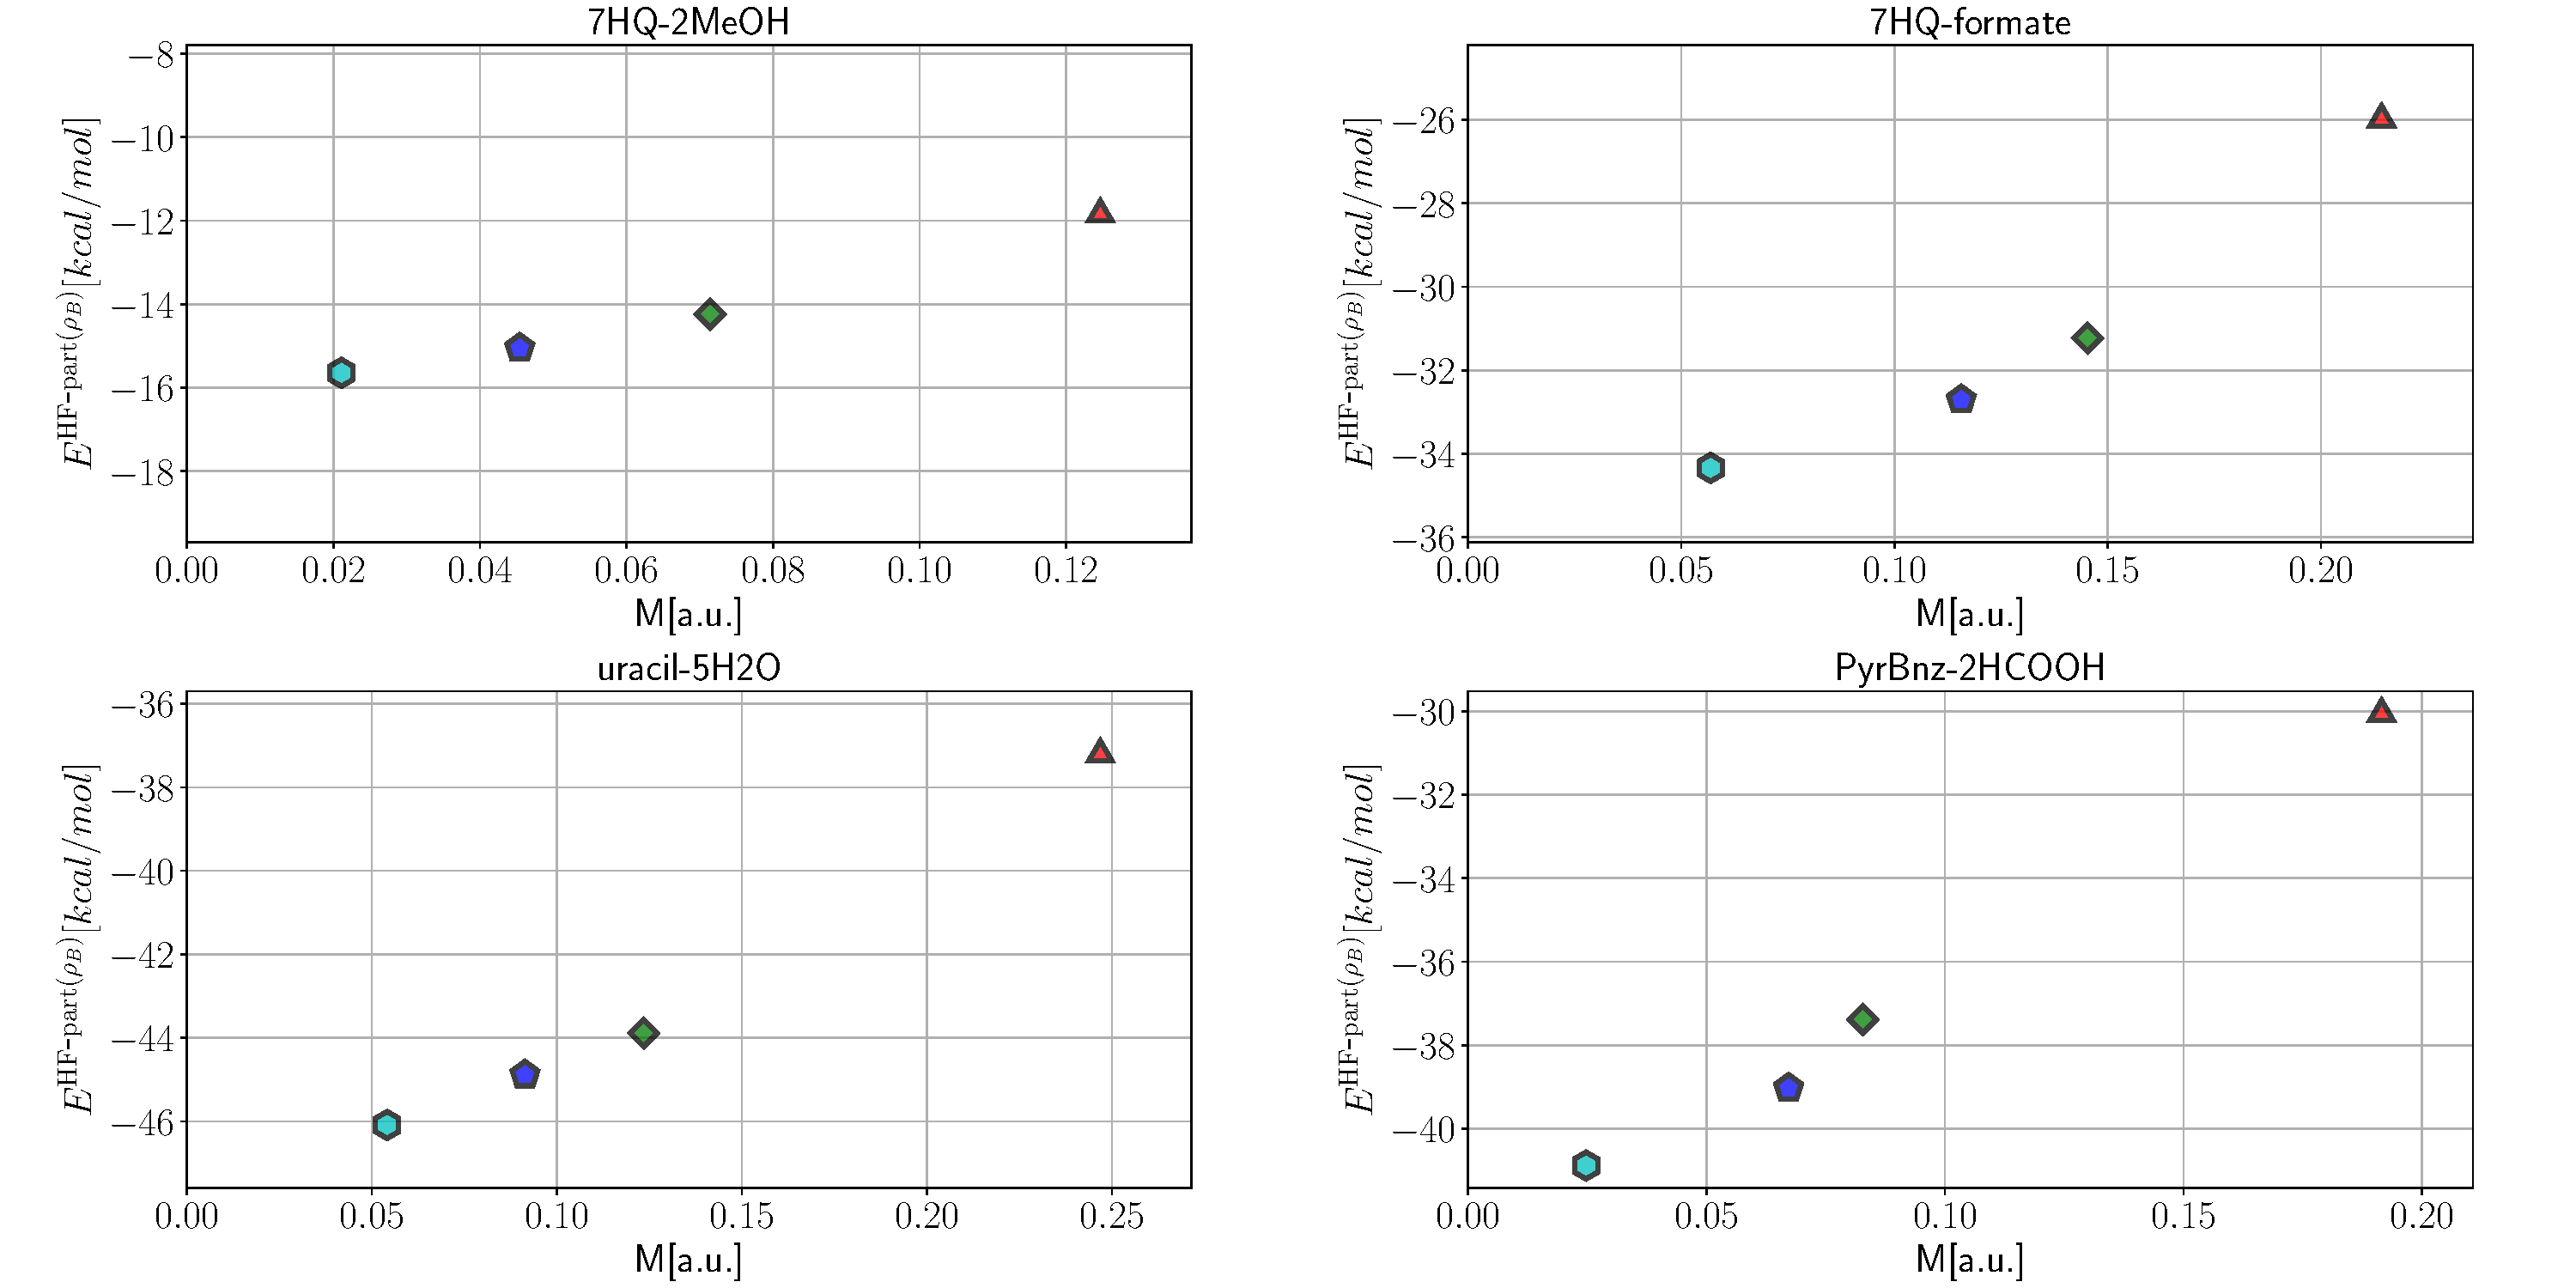
\includegraphics[width=1.0\linewidth]{M_vs_HF.png}
\caption{Integrated negative density $M$ and the FDET-HF component of the FDET-MP2 interaction energy for various choices of $\rho_B(\mathbf{r})$:  a) $\rho_B^{isol}(\mathbf{r})$ (orange triangles), b) $\rho_B^{FAT}(\mathbf{r})$ (light blue hexagons), c) $\rho_B^{pp(Mulliken)}(\mathbf{r})$ (green diamonds), and d) $\rho_B^{pp(ChelPG)}(\mathbf{r})$ (dark blue pentagons). Data obtained using the monomer expansion. Horizontal lies indicate the reference interaction energy.}
\label{fig:M_VS_HF}
\end{figure}



\subsection{Self-consistency of the embedded wavefunction and embedding potential}\label{sect:self_consistency}
The basic FDET equality given in Eq. \ref{eq:nfund}, holds only if the optimal embedded wavefunction is consistent with the embedding potential (the latter depends on the embedded wavefunction).  Assuring self-consistency involves solving repetitively the quantum $N_A$-electron problem. Linearisation of $\tilde{E}_{xcT}^{nad}[\rho_A,\rho_B]$ in  
$\rho_A(\mathbf{r})$ makes it possible to avoid it \cite{Zech2015}. 
\begin{equation}
 \tilde{E}_{xcT}^{nad}[\rho_A,\rho_B] \approx  \tilde{E}_{xcT}^{nad}[\rho_A^{init},\rho_B] + \Delta^{lin}[\rho_A,\rho_A^{init},\rho_B] %+ O^2( \rho_A -  \rho_A^{init}) 
,\label{eq:linearisation}
\end{equation}
where:
\begin{equation}\label{eq:delta_lin}
        \Delta^{lin}[\rho_A,\rho_A^{init},\rho_B]  = \displaystyle\int \left( \rho_A(\mathbf{r}) -  \rho_A^{init}(\mathbf{r}) \right) \frac{\delta \tilde{E}_{xcT}^{nad}[\rho_A, \rho_B]}{\delta \rho_A(\mathbf{r})}
 \Bigg \vert_{\rho_A^{init}}
 \mathrm{d}\mathbf{r}.    
\end{equation}

Linearisation of $\tilde{E}_{xcT}^{nad}[\rho_A,\rho_B]$  
%Eq. \ref{eq:linearisation}, 
was used in Ref. \citenum{Zech2015} to deal with the issue of non-orthogonality of embedded wavefunctions  for different electronic states. In such a case, $\rho_A^{init}(\mathbf{r})$ corresponds to the ground-state density whereas $\rho_A(\mathbf{r})$ to one of the excited states. 
In the present work, Eq. \ref{eq:linearisation} is  used  for another purpose - to accelerate obtaining  the self-consistent ground-state embedded wavefunction. 
%For instance in a series of calculations are made for slightly different  $\rho_B(\mathbf{r})$. 
In calculations, in which $\rho_B(\mathbf{r})$ was optimised,  the freeze-and-thaw  iterative procedure was used \cite{Wesolowski1996a}. 
In the subsequent iteration of this procedure, the indices $A$ and $B$ exchange their role in the FDET equations.
%
%In the present work,  the  freeze-and-thaw iterations are used to optimise $\rho_B(\mathbf{r})$. 
Since the optimised densities $\rho_A(\mathbf{r})$ do not change significantly in the subsequent iterations, the density obtained in a given freeze-and-thaw iteration is used as  $\rho_A^{init}(\mathbf{r})$ in the linearized expression for $\tilde{E}_{xcT}^{nad}[\rho_A,\rho_B]$ in the subsequent iteration. 
Although the embedding potential and the optimal density are not consistent at intermediate steps, the consistency is reached in the final iteration.
